\begin{frame}{\(n\)-cubes}

\begin{columns}[T,onlytextwidth]
	\begin{column}{0.5\textwidth}
		\centering
        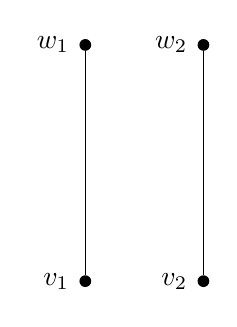
\begin{tikzpicture}[scale=3]
            \node[circle, fill, inner sep=1.5pt, label=left:\(v_1\)] (v1) at (0,0) {};
            \node[circle, fill, inner sep=1.5pt, label=left:\(w_1\)] (w1) at (0,1) {};
            \draw (v1) -- (w1);

            \node[circle, fill, inner sep=1.5pt, label=left:\(v_2\)] (v2) at (0.5,0) {};
            \node[circle, fill, inner sep=1.5pt, label=left:\(w_2\)] (w2) at (0.5,1) {};
            \draw (v2) -- (w2);


        \end{tikzpicture}
        
		\scriptsize \(\Gamma\) is two disjoint edges.
	\end{column}

	\begin{column}{0.5\textwidth}
		\centering
        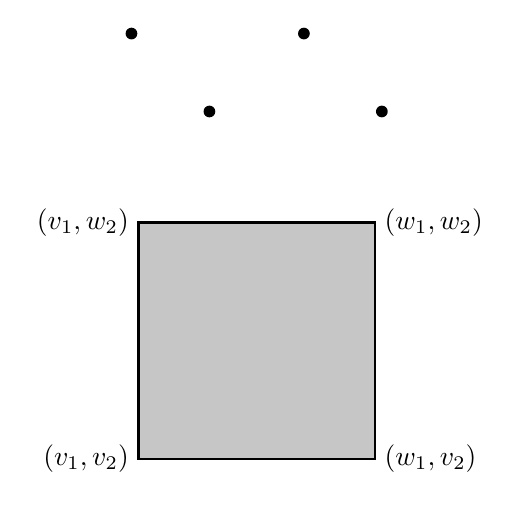
\begin{tikzpicture}[scale=3]
            \fill[gray, opacity=0.45] (0,-.3) rectangle (1,.7);
            \draw[thick] (0,-.3) rectangle (1,.7);
            \node[left] (v1v1) at (0,-.3) {\((v_1, v_2)\)};
            \node[right] (w1w1) at (1,.7) {\((w_1, w_2)\)};
            \node[left] (v1w1) at (0,.7) {\((v_1, w_2)\)};
            \node[right] (w1v1) at (1,-.3) {\((w_1, v_2)\)};


            \node[circle, fill, inner sep=1.5pt] (v1w1) at (-.03,1.5) {};
            \node[circle, fill, inner sep=1.5pt] (w1v1) at (.3,1.17) {};
            \node[circle, fill, inner sep=1.5pt] (v2w2) at (.7,1.5) {};
            \node[circle, fill, inner sep=1.5pt] (w2v2) at (1.03,1.17) {};
        \end{tikzpicture}

		\scriptsize \(\DConf_2(\Gamma)\).
    \end{column}
\end{columns}

\end{frame}